\chapter{The MODES-SNM Project}
MODES-SNM (MOdular DEtection System for Special Nuclear Material) is a collaborative project concerned with tackling nuclear threats with a compact and portable approach \cite{website:modes}. A modular and mobile system design is considered with the capability of detecting and identifying radioactive and Special Nuclear Material (SNM). Within a period of only 30 months the project aimed to produce and test a fully integrated prototype of the system. Unlike LAGUNA-LBNO, this project is considerably smaller both financially and physically, however it has the potential to impact, not only the scientific community, but also the whole of modern society, enormously. This chapter presents an overview of the project with an introduction to potential uses and other current technologies.

\section{Detecting Special Nuclear Materials}
%Current systems are primitive in the combat against such hazards as nuclear devices, dirty bombs and SNM. 
Nuclear terrorism is a modern day threat to society. Highly enriched uranium ($^{235}$U) and weapons grade plutonium ($^{239}$Pu) are SNM. Illicit trafficking of such material can suggest the intent to make or use Improvised Nuclear Devices (IND). It is understood that quantities of the order of 8 kg of plutonium or 25 kg of highly enriched uranium are required to build an IND \cite{modesIAEABorder}. 
%The US Domestic Nuclear Office (DNDO) has set targets of $\sim$2 kg (100 m$^{3}$) of each material as quantities for detection [ref here].

SNM are high emitters of $\alpha$ and $\beta$ particles, gammas and neutrons. With the former being stopped by a few centimetres of air, detection of the latter two provides the only viable indication of SNM. Detection of gammas can provide a strong signature of radioactive material, but they are heavily effected by source shielding. Shielding or masking of sources impedes dramatically on the ability to detect SNM and results in losses of sensitivity in detectors. It is therefore necessary to have a system that is sensitive to shielded sources and employs an effective analysis to identify potential threats.

\subsection{Current Technologies}
Most modern technologies use gamma detectors to monitor radiation threats with the inclusion of optional neutron detectors for SNM. Examples are discussed in the following sections.
\subsubsection{Gamma Detection}
The three main processes in which gamma rays are detected are via the photoelectric effect, Compton scattering or pair production. These interactions all lead to the production of energetic electrons via partial or complete energy transfer from the photon. %Figure \ref{fig:sodiumIodideXSec} shows the cross sections of these processes on a the most popular of gamma detection media, Sodium Iodide (NaI). 

%\begin{figure}[htbp]
%\begin{center}
%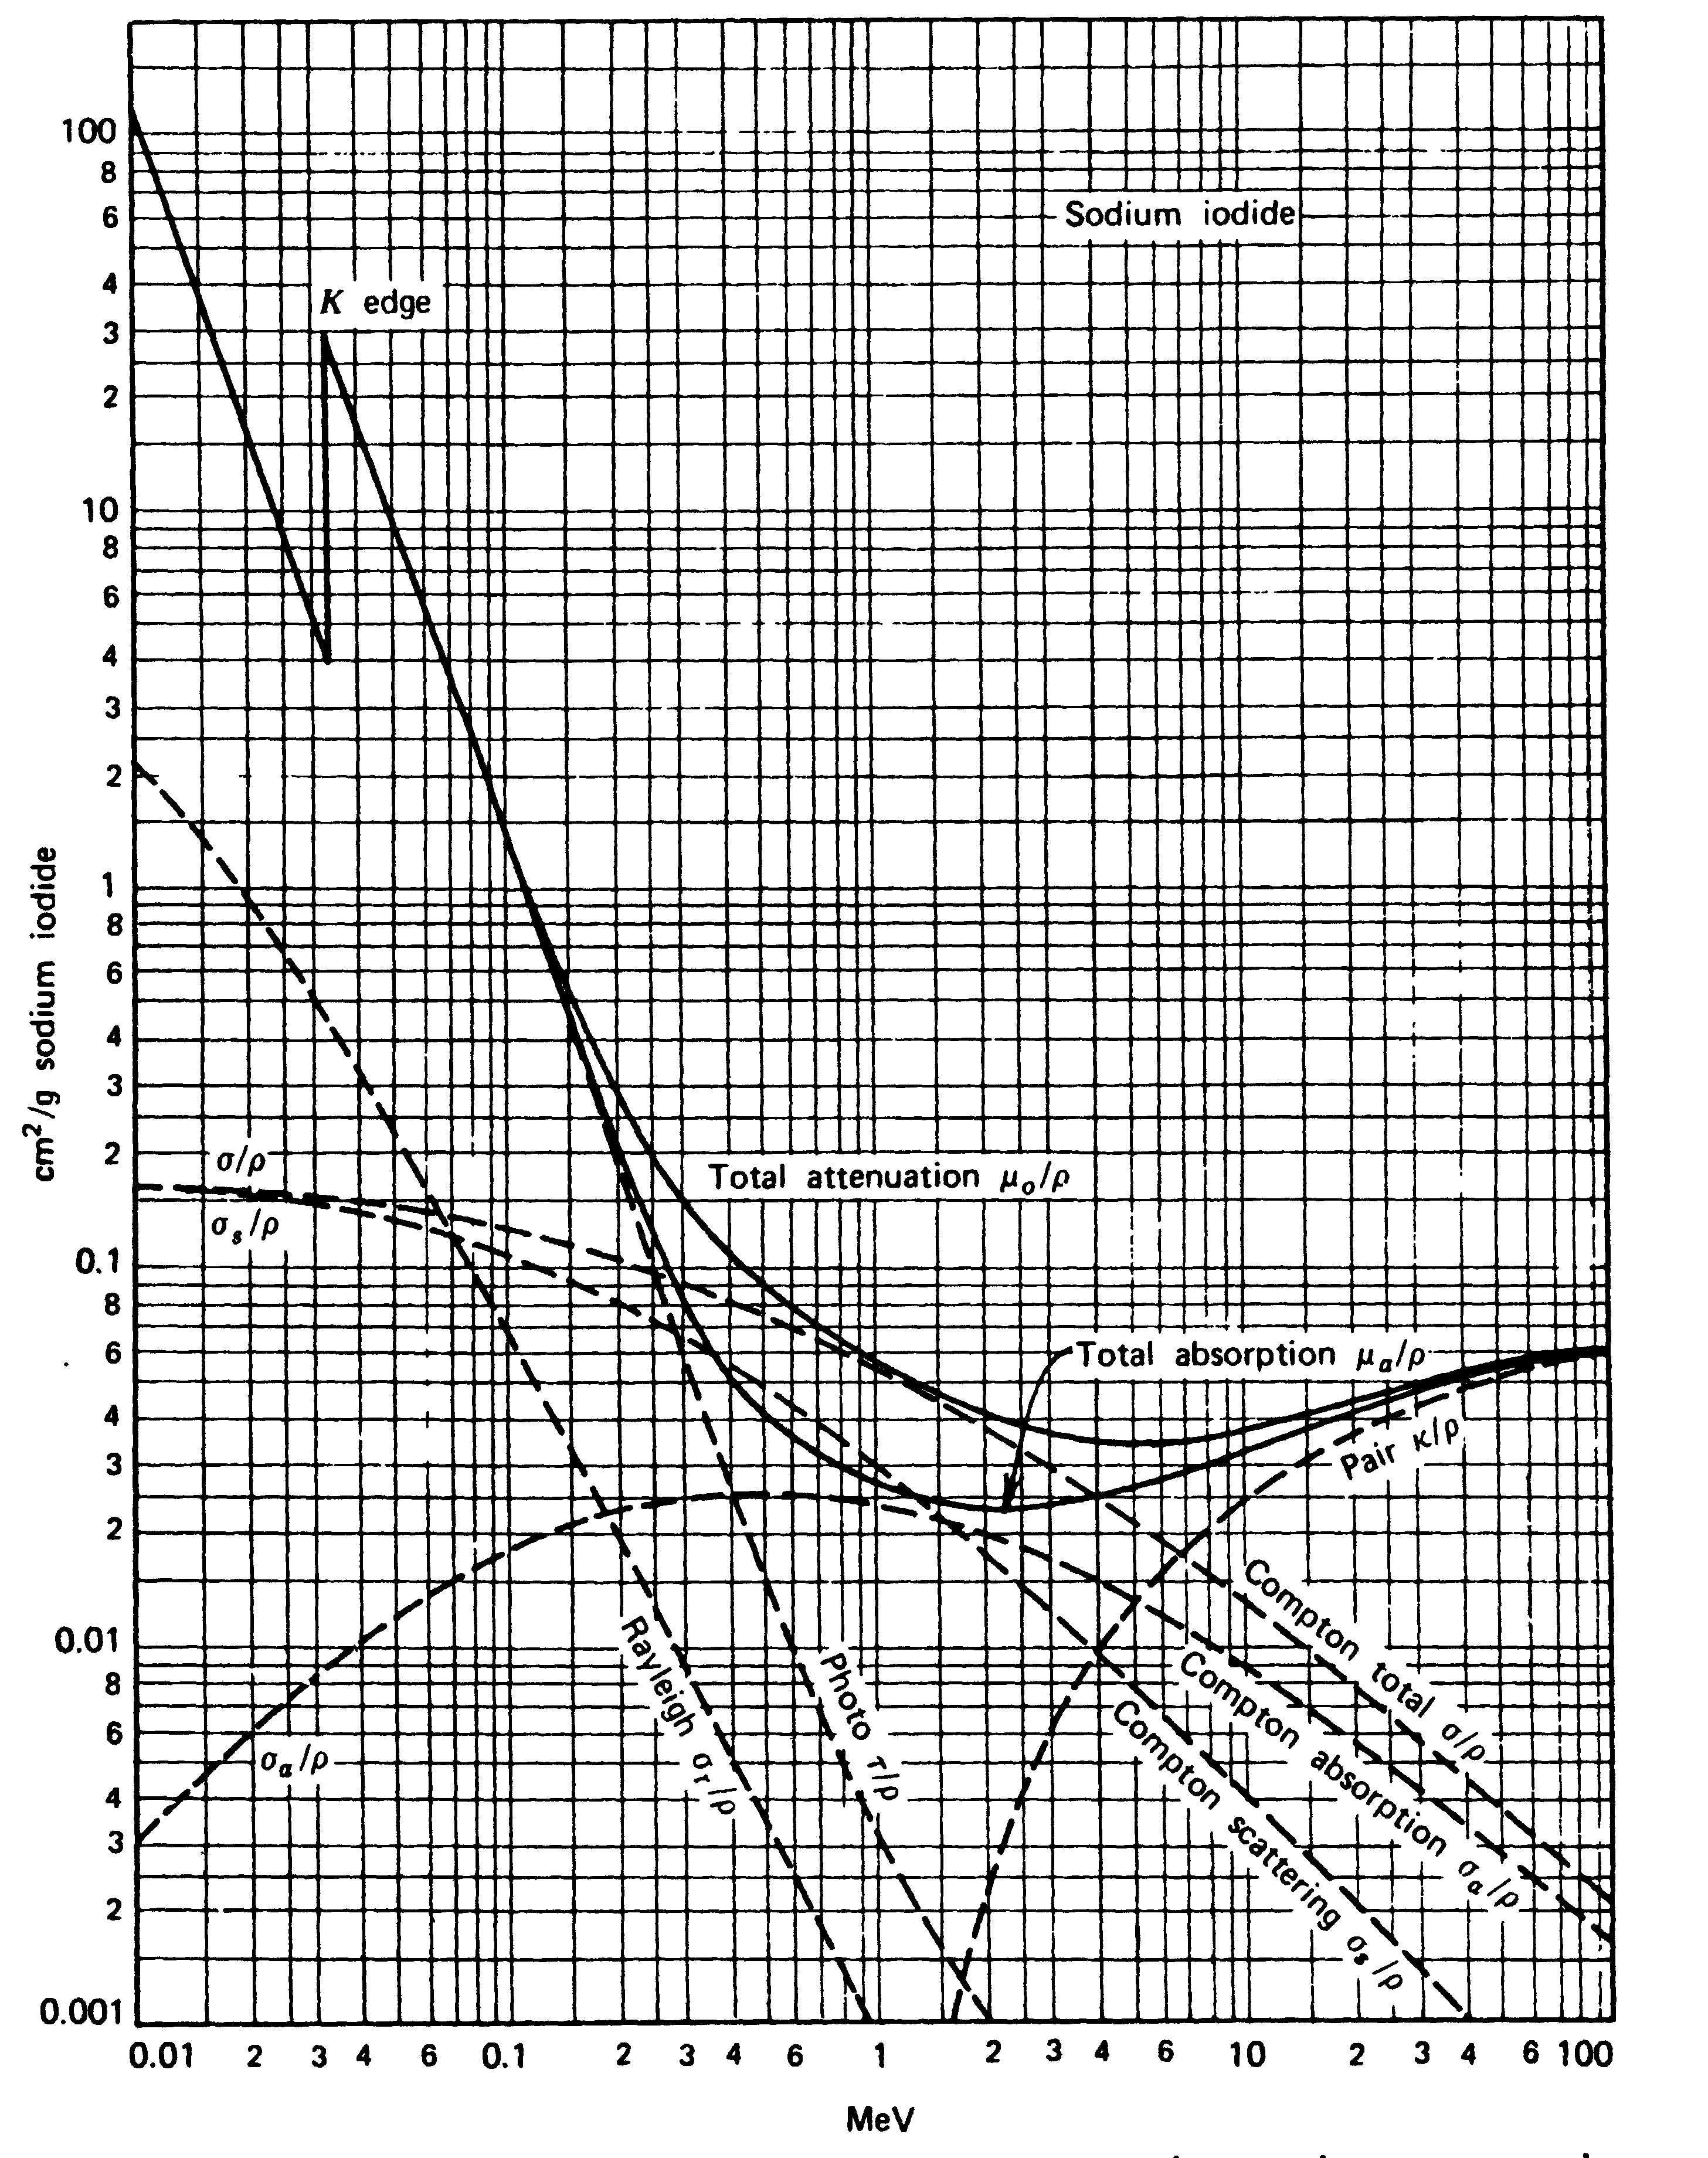
\includegraphics[width=120mm]{Chapter5/figures/sodiumIodideGammaXSec.png}
%\caption{The energy dependance on certain gamma ray interaction processes. Plot taken from \cite{knollRadiation}.}
%\label{fig:sodiumIodideXSec}
%\end{center}
%\end{figure}

NaI detectors are inorganic scintillator detectors that are the most frequently used technology for gamma ray detection. Inorganic scintillators are preferred to their organic counterpart due to the light yield production ($\sim$40,000 $\gamma$/MeV) but are quite slow in comparison \cite{knollRadiation}. The energy resolution of inorganic detectors are also fairly poor, with Full Width Half maximum (FWHM) values of between 5-15\% for sources within the 0.1 - 1 keV range. 

In order to gain better photon production efficiencies, impurities are added in the form of an activator. Due to these added impurities the energy band structure of the crystal lattice is altered and yields previously forbidden energy bands between the conduction and valence bands. In turn this results in the emission of visible fluorescent photons that can be collected. For NaI detectors, thallium (Tl) is the activator. NaI(Tl) technologies offer good detector efficiencies \cite{knollRadiation}, as they can be produced in large crystals, good energy resolutions (when compared with other scintillator materials) and high light yields.

High Purity Germanium (HPGe) semiconductor detectors are also common place in gamma spectroscopy. Unlike scintillator detectors they rely on the detection of charge carriers produced from photon interactions. A photon upon energy deposition will move an electron to the conduction band producing a hole in the valence band. Applying an electric field will provide a net migration of the charge carriers which is then read out. Devices using HPGe boast very good energy resolutions in comparison to NaI(TI) but are limited to small sizes as fabrication of very high purity germanium is difficult. As a result detection efficiency can be orders of magnitude worse than NaI detectors.

The far superior energy resolution of HPGe devices makes them extremely useful for resolving close gamma peaks in the energy spectra. NaI devices are poor in this respect. Although this is a very favourable trait a trade off occurs with detection efficiency, and for some applications it may be favourable to use NaI technology. Other devices such as plastic scintillator detectors are also used for gamma ray spectroscopy, however NaI and HPGe devices are by far the most common.
 
\subsubsection{Neutron Detection}
The detection of neutrons falls into two categories: slow and fast neutron detection. 
Almost all current technologies on the market for slow neutron detection rely on neutron capture. The subsequent recoiling nucleus, proton or alpha particle is then observed and measured in the detector. Technologies implementing this process however offer no knowledge of the incident neutron energy.

Materials such as $^{3}$He, $^{6}$Li, $^{10}$B and $^{157}$Gd are renowned for their high neutron absorption cross section, which can be seen in figure \ref{fig:neutronXSec1}. Using these materials as the target medium then allows detectors to have smaller active volumes and can be used in smaller devices.

\begin{figure}[htbp]
\begin{center}
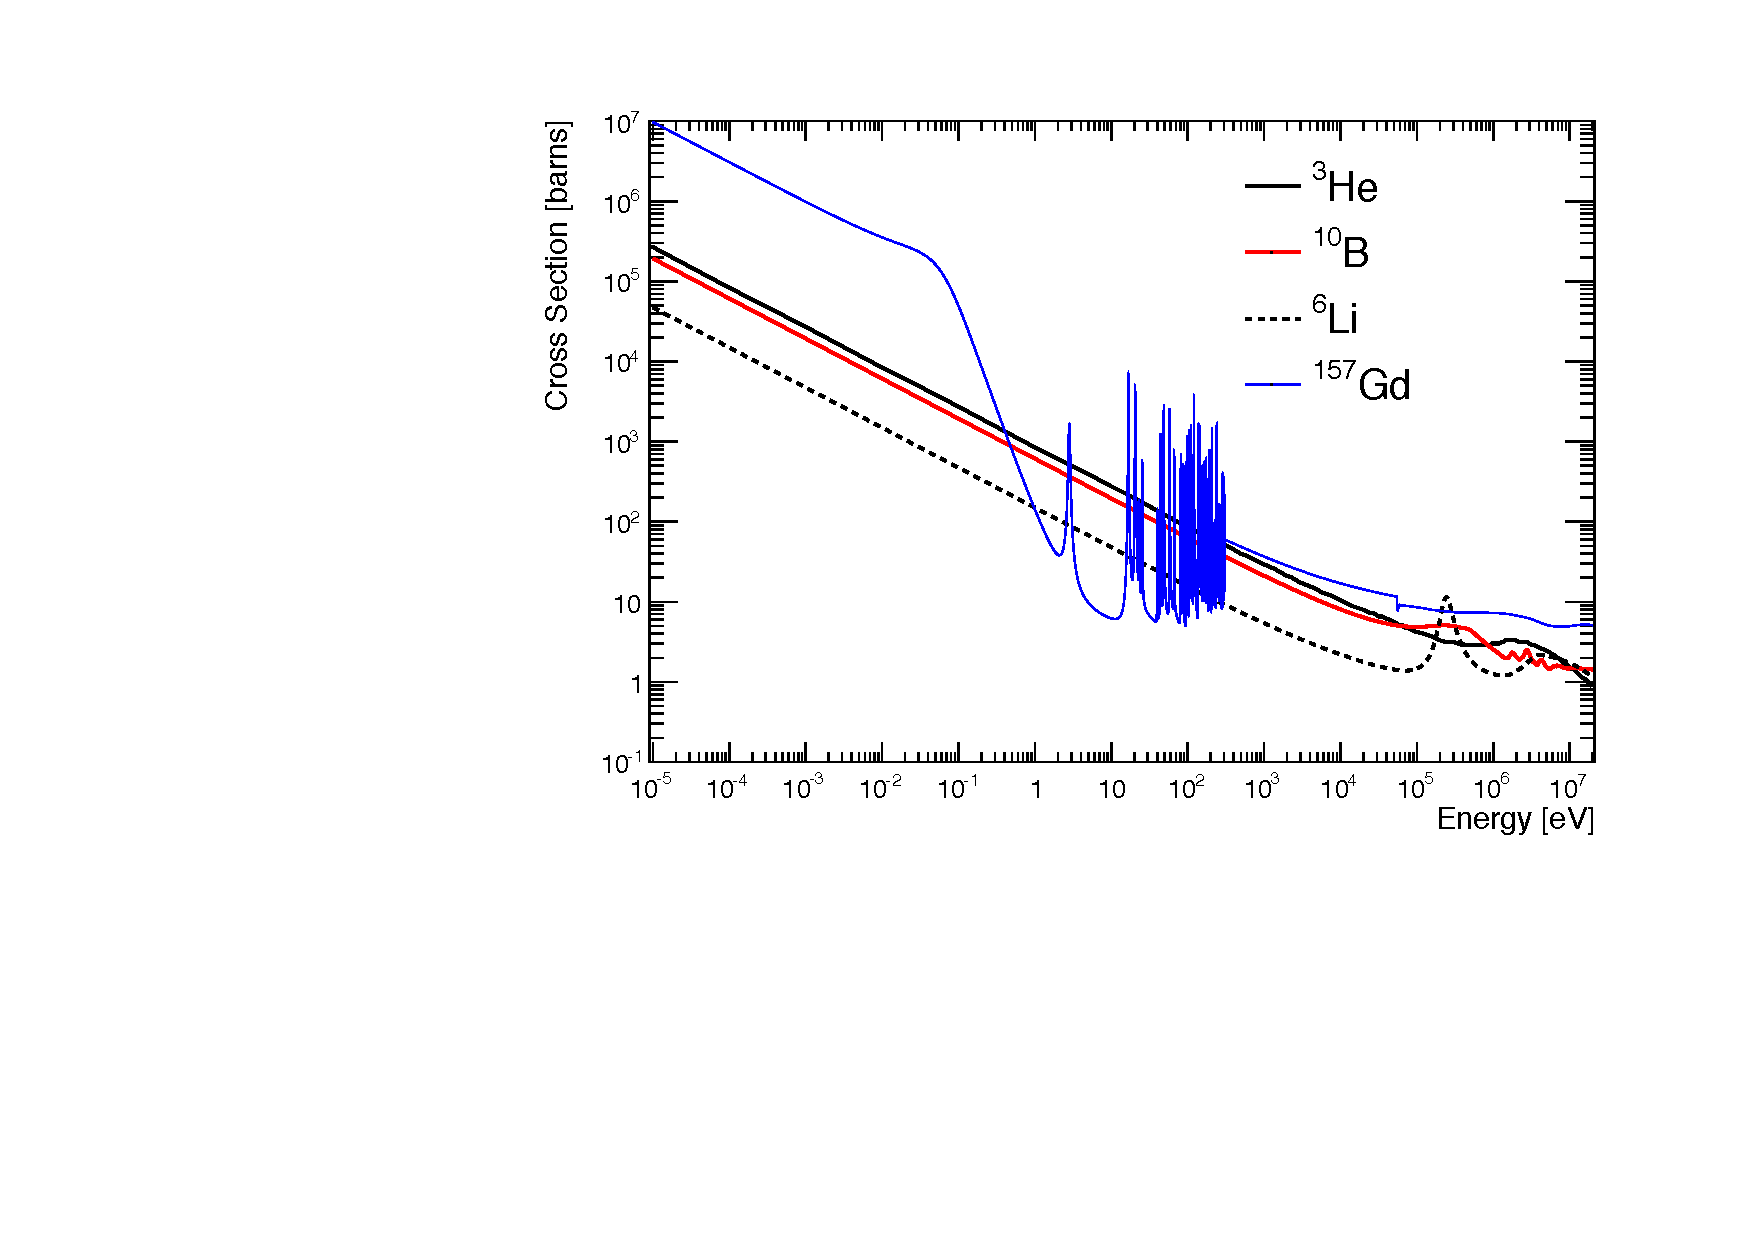
\includegraphics[width=120mm]{Chapter5/figures/neutronSlowMediaTotalXSec2.pdf}
\caption{The neutron total cross sections for $^{3}$He, $^{6}$Li, $^{10}$B and $^{157}$Gd. Data taken from the ENDF-VII.1 library \cite{endfLibrary}.}
\label{fig:neutronXSec1}
\end{center}
\end{figure}

Fast neutron detection relies on elastic scattering which causes nuclear recoil, in turn creating ionisation. Shown previously in equation \ref{eq:neutronScatter}, it can be noticed that the ratio $T_{A}/T_{n}$ can only give a 100\% energy transfer for hydrogen. Due to these restrictions hydrogen is the predominately favoured technology for fast neutron detection. $^{3}$He is also used as it can allow for up to 75\% energy transfer per elastic scatter. It is clear from this, contrary to slow neutrons, that the energy of the incident neutron can be determined given an accurate measurement of the recoil nucleus energy deposition.

\subsection{Current Systems}
Several types of radioactive detection systems are currently employed at customs and borders worldwide to help combat potential nuclear threats. Most offer passive and non intrusive methods of screening and fall within three categories of instruments; fixed/automatic, portable/hand-held, and pocket-type \cite{modesIAEABorder}.

\subsubsection{Fixed and Automatic Systems}
These types of instrument are commonly deployed as primary detector systems to act as the first barrier against nuclear threats. Such instruments are automatic and have the ability to screen large volumes of traffic. The continuous measurement of the gamma and neutron background levels and readjustment of the alarm threshold maintains a statistically constant false alarm rate. Occupancy sensors are then required to inform the system when to measure radiation levels of passing traffic. Background measurements are compared to the occupied measurement and an alarm is declared if it falls outside preset thresholds. 

Radiation Portal Monitors (RPM) are currently the most prevalent of this type of technology, shown in figure \ref{fig:RPMLorry}. They are usually arranged in two parallel pillars placed either side of passing traffic. In this arrangement the system can probe cargo closely and symmetrically. Most RPMs will monitor both gamma and neutron rates. The most frequent technology for detection of the former is NaI scintillating crystals, while the latter relies on $^{3}$He gas detectors. Large arrays of the detectors then form the basis of the RPM.
%However due to recent supply shortages of $^{3}$He it is no longer being considered for new designs.

\begin{figure}[htbp]
\begin{center}
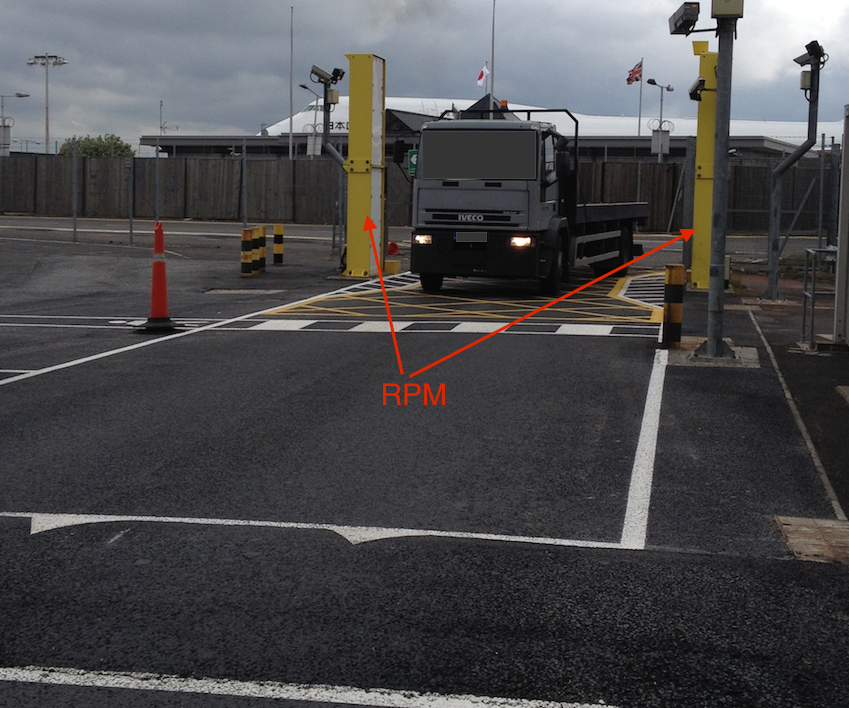
\includegraphics[width=80mm]{Chapter5/figures/rpm2.png}
\caption{An image of a fixed RPM used at an airport with a cargo truck passing through it. The RPM is the large yellow detectors placed either side of the passing vehicle.}
\label{fig:RPMLorry}
\end{center}
\end{figure}

\subsubsection{Portable Systems}
Secondary detection systems are employed for use if cargo or vehicles raise suspicion from the primary system. This usually involves the deployment of portable or handheld systems. There are many variations of these particular systems but they all use common technology similar to the RPM, NaI detectors for gammas and $^{3}$He or $^{6}$Li for neutron detection. These type of detectors measure dose-rates with some more sophisticated systems able to perform identification. They can be deployed as primary detectors but are usually less sensitive due to the reduction of the active volume, especially for hand held devices. Longer exposure times compensate for the reduction of the active volume, and are why they work well as secondary devices.

\subsubsection{Pocket-Type Systems}
When only concerned with gamma radiation rates, these systems are cheap to produce and easily usable. However due to their size, they can only measure dose rates and cannot perform radionuclide identification. Such devices are commonly used to monitor individuals personal dose rates when exposed to potential radioactive areas, such as customs and border personnel. Only scintillation detectors are sensitive enough for use in these devices.

\subsubsection{Issues}
The are some severe issues with the current systems and their associated technologies. The generation of false alarms due to Naturally Occurring Radioactive Material (NORM) or other non threatening radioactive sources is a continuous nuisance. Reports suggest that 1\% of alarms are due to NORM \cite{modesNORM}, and with large volumes of traffic it becomes more than an inconvenience. Other innocent alarms can originate from medical treatment (radio-pharmaceuticals), with $\sim$1 in every 2600 people crossing the U.S border triggering such an alarm \cite{modesRPMFalse}. These current levels of innocent alarm rates are a very costly disruption while monitoring the trafficking of illicit material. The sensitivity of these systems is also under scrutiny with new systems required to detect shielded or masked neutron sources. Coupled with the worldwide shortage of $^{3}$He new technologies and techniques must be developed.
%RPMs and other similar systems produce an alarm when the ionising radiation detected exceeds the natural background level.
%contributes to $\sim$1 in every 2600 U.S border controls.

\subsection{The Abundance of $^{4}$He}
With $^{3}$He suffering from a severe supply shortage \cite{helium3Shortage}, other candidates for detection of neutrons are required. A potential candidate for its replacement is $^{4}$He \cite{helium4Detectors}. Although $^{3}$He has a large cross section for neutron capture, at higher energies ($\sim$500 keV and above) $^{4}$He has a larger cross section due to elastic scattering. This can be seen in figure \ref{fig:heliumCrossSection}. Utilising this improved cross section requires a different detection technique as neutrons will elastically scatter off of $^{4}$He atoms in the detection medium and the subsequent recoil of the $^{4}$He atom will cause ionisation in the medium (gas), in turn producing scintillation light which can be collected. The number of collected photons is then proportional to the energy deposited by the incident neutron. Coupled with a high scintillation light yield of $\sim$18,000 VUV makes this technique possible. 

This is a powerful technique when used for the detection of fast neutrons, especially for SNM, but for slow neutrons the difference in cross section is large, with a factor of $\sim$10,000 less at $\sim$1 eV. However adding a coating of $^{6}$Li or another absorber then allows for neutron capture and the alpha emission can be seen in the active volume. 

\begin{figure}[htbp]
\begin{center}
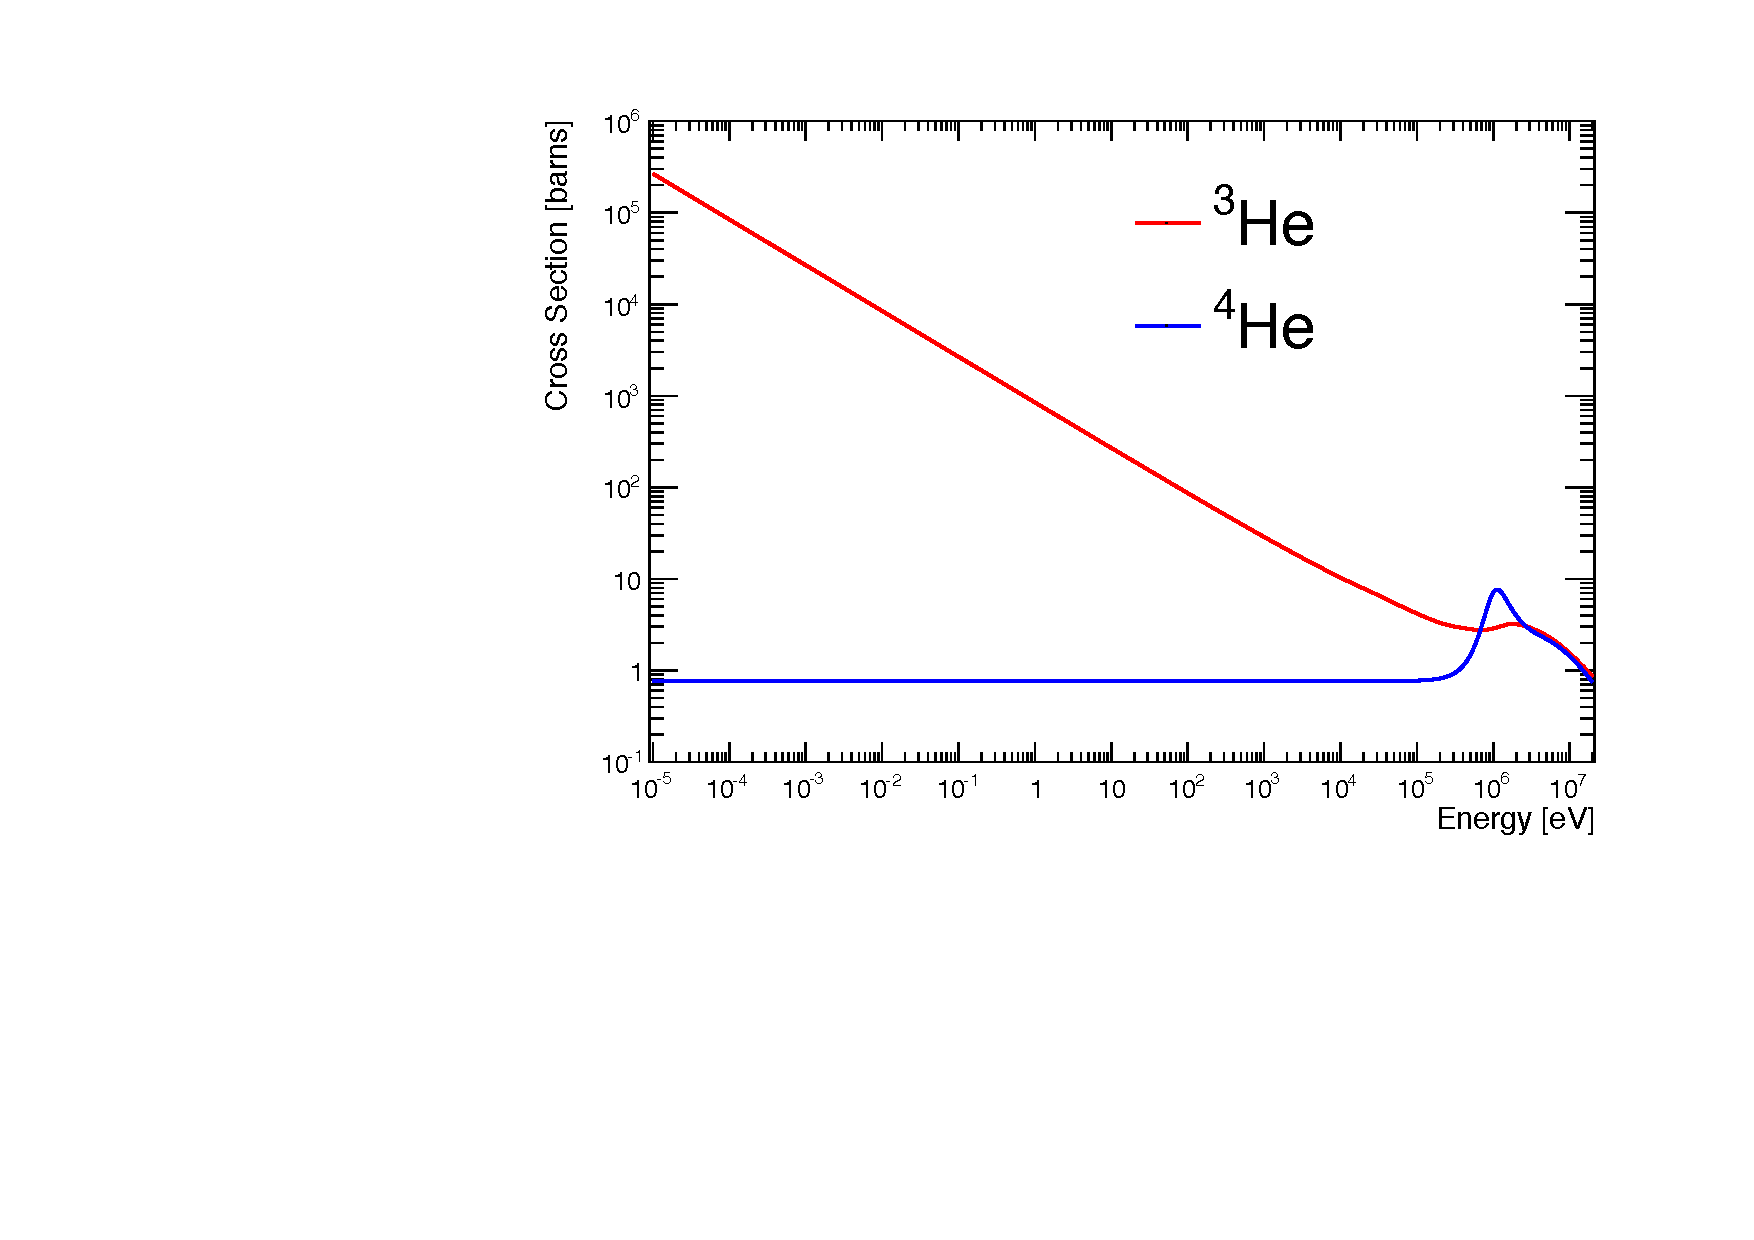
\includegraphics[width=100mm]{Chapter5/figures/neutronHeliumTotalXSec.pdf}
\caption{The neutron total cross sections for $^{3}$He and $^{4}$He. Data taken from the ENDF-VII.1 library \cite{endfLibrary}.}
\label{fig:heliumCrossSection}
\end{center}
\end{figure}

%$^{4}$He is a fairly good scintillator, with similar light yields to NaI crystals \cite{}. 

\section{The MODES-SNM System}
The MODES-SNM consortium was conceived in January 2012 in order to develop new technology and integrate it into a new generation of radiation detector systems. It consists of the following participants: University of Liverpool (UNILIV); Universit\`{a} degli Studi di Padova, Italy (UNIPD); ARKTIS Radiation Detectors Ltd, Switzerland (ARKTIS); Narodowe Centrum Bada\'{n} J\c{a}drowych - National Centre for Nuclear Research, Poland (NCBJ); Eidgen\"{o}ssische Technische Hochschule Z\"{u}rich, Switzerland (ETHZ); Costruzioni Apparecchiature Elettroniche Nucleari, Italy (CAEN); Universit\`{a} degli Studi dell'Insubria, Italy (UINS); Revenue Commissioners, Ireland (RC). 
%Together the collaboration aims to use their individual expertise to collectively tackle....  

\subsection{Sensitivity Requirements}
Certain minimal requirements are imposed on the prototype based on the sensitivity recommendations set by the International Atomic Energy Agency (IAEA) \cite{modesIAEABorder}. Specific requirements imposed from the International Electrotechnical Commission (IEC) are integrated into these also \cite{IEC62244}. With MODES-SNM being a portable/mobile system with the option to function as a fixed detector, like an RPM, it must support both mobile and fixed (RPM) criteria.

A true alarm is defined as an alarm that is raised in the presence of a radioactive source. Contrary to this a false alarm is an alarm raised when no radioactive source is present and the background is stable (false positive). The true alarm rate should be at or greater than 96/100 trials, corresponding to a probability of detection of 90\% at a 95\% confidence level \cite{passFailStats}. The false alarm rate (FAR) should not exceed 1 alarm per hour, with the detector operating in stationary mode.

For gamma detection an alarm should be generated for a source of dose rate of 0.05 $\mu$Sv/h at a minimum distance of 1 m separation from the instrument passing by with a speed of 0.5 m/s (1.8 km/h). Specifically this requirement shall be met for sources of $^{241}$Am, $^{137}$Cs and $^{60}$Co, corresponding to an energy range of 50 keV to 1.5 MeV. The activities of these sources are listed in table \ref{tab:gammaSourcesDetection}, with their corresponding gamma  emission energies and the required activities for a dose rate of 0.05 $\mu$Sv/h at 1 m distance.

\begin{table}[!htbp]
\begin{center}
	\begin{tabular}{l*{2}{c}r}
	\hline
	 \hline
	 Source & Gamma Energy & Required Activity \\
    	\hline
    	$^{60}$Co	 & 1.17, 1.33 MeV &  160 kBq\\
    	$^{137}$Cs & 662 keV & 660 kBq \\
    	$^{241}$Am & 59.5 keV & 13 MBq \\
    	\hline
    	\hline
  	\end{tabular}
	\caption{The gamma sources with their associated energies and activities required to produce a dose rate of 0.05 $\mu$Sv/h at 1 m distance.}
    	\label{tab:gammaSourcesDetection}
\end{center}
\end{table}

For neutron detection an alarm should be generated for a $^{252}$Cf source, of activity 1.2 $\times$ 10$^{4}$ neutrons/s, whilst in motion at a speed of 0.5 m/s (1.8 km/h). Again the distance between the source and the system should be no less than 1 m. This is equivalent to a static rate of 0.1 neutrons cm$^{-2}$s$^{-1}$ at 1 m distance. For stationary screening, this requirement is increased such that the activity is reduced to $\sim$5 $\times$ 10$^{3}$ neutrons/s. This corresponds to 0.04 neutrons cm$^{-2}$s$^{-1}$ at 1 m distance. 

\subsection{Nuclide Identification Requirements}
In addition to the sensitivity requirements, radioactive source identification requirements are also set by the IEC \cite{IEC62244}. The identification of the following radioactive sources: $^{152}$Eu, $^{133}$Ba, $^{22}$Na (PET-type source), $^{51}$Cr, $^{57}$Co, $^{60}$Co, $^{137}$Cs, $^{241}$Am should be performed within a 60 s exposure from rates of 50 nSv/h to 5.0 $\mu$Sv/h.

\subsection{The Detector Concept}
The prototype system implements both gamma and neutron detection, with the latter consisting of thermal and fast neutrons. The technology behind all 3 detectors relies on high pressure noble gases used as scintillation volumes. $^{4}$He is implemented for neutron detection while Xe is used for gamma detection. Design and development of detectors incorporating these gases have been performed by ARKTIS prior to and along side the MODES-SNM project. The Fast Neutron Detectors (FND) have been developed independently prior to the MODES-SNM collaboration \cite{helium4Detectors}, whereas the development of the Slow Neutron Detectors (SND) and Gamma Detectors (GD) are part of the MODES-SNM project \cite{xenonScintDetectors}. The SND and GD designs follow from an evolution of the design of the FND. 

The 3 various types of detector all follow the same design. Each type consists of a cylindrical pressure vessel filled with an active gas of either $^{4}$He or Xe. Lining the inside of the tubes exists a WaveLength Shifter (WLS) to reradiate scintillation light to the Vacuum Ultra Violet (VUV) range. Photo Multiplier Tubes (PMTs) are placed at either end of the tube with VUV transparent windows serving as the intermediary between the tube and the PMT for light collection. This is shown in figure \ref{fig:detectorConcept}.

\begin{figure}[htbp]
\begin{center}
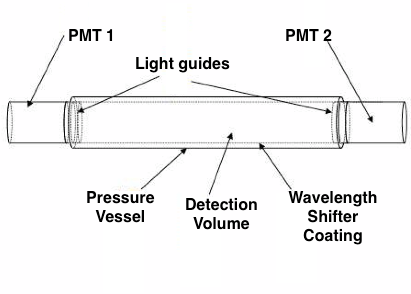
\includegraphics[width=100mm]{Chapter5/figures/neutronDetectorLabelled2.png}
\caption{The basic design of the detectors used in MODES-SNM.}
\label{fig:detectorConcept}
\end{center}
\end{figure}

This detector design does not allow for recirculation of the gas which is a common method of purifying the gas. As a result high purity is required to achieve high scintillation yields. 

\subsubsection{Fast Neutron Detectors}
With low atomic number (Z=2) and low mass number (A=4), $^{4}$He is well suited as a medium for neutron detection. Due to kinematic restrictions, only 64\% of the incident neutrons kinetic energy can be transferred to the nucleus per elastic scatter, calculated from equation \ref{eq:neutronScatter}. Although not as good as hydrogen it is the highest energy transfer for the nobel gases. helium

The FND contain pressurised $^{4}$He at $\sim$180 bar in tubes of active volume of $\sim$714 cm$^{3}$ (470 mm length and 44 mm diameter). At this pressure the corresponding density is 0.03 gcm$^{-3}$ at room temperature. Studies close to this pressure at 200 bar have shown $^{4}$He is a fairly good scintillator with a light yield of approximately 18,000 VUV photons / MeV deposited by neutrons \cite{helium4Detectors} \cite{knollRadiation}. That is just less than half that of NaI detectors ($\sim$40,000). The scintillation light produced in $^{4}$He has a wavelength of the order of 70 nm ($\sim$18 eV).

Gamma rejection is important for neutron detection in order to discrimination against source masking or NORM radiation. helium is excellent for this due to four main reasons:

\begin{itemize}
	\item A low atomic number results in low sensitivity to gammas, having a cross section of a factor $\sim$20 less than neutrons around $\sim$1 MeV. 
	\item Low energy deposition from recoiling electrons in the gas due to gamma interactions, hence low ionisation.
	\item Low light yield for gamma interactions due to electron recoil, as opposed to nuclear recoil for neutrons. Recombination of electron-ion pairs in pressurised $^{4}$He is considered as an inefficient process.
	\item Pulse Shape Discrimination (PSD) is a powerful tool that can be applied to scintillation signals, due to the fast and slow components of scintillation light.
\end{itemize}

Given that the average exposure time of the detector is between 2-3 seconds, a conservative limit of R = 10 neutrons s$^{-1}$ is assumed. To estimate the number of required detectors, N, equation \ref{eq:eventRate} is used. Table \ref{tab:neutronCfNumbers} shows the parameters used in the calculation with some extracted from sources \cite{helium4Detectors},\cite{endfLibrary} and \cite{cf252Neutrons}.

\begin{equation}
	N = \frac{mR}{\rho V_{0}\sigma \phi}
	\label{eq:eventRate}
\end{equation}

\begin{table}[!htbp]
	\begin{center}
	\begin{tabular}{l*{2}{c}r}
	\hline
	 \hline
	 Parameter & Value & Description \\
    	\hline
	E & 1 MeV & Peak neutron energy from $^{252}$Cf spontaneous fission \cite{cf252Neutrons} \\
    	$\sigma$ & $\sim$10$^{-27}$ m$^{2}$ & Neutron cross section on $^{4}$He at peak energy \cite{endfLibrary}\\
	m & 6.68 $\times$ 10$^{-27}$ kg & $^{4}$He atomic mass \\
	R & 10 n/s & Neutron detection rate \\
	$V_{0}$ & $\sim$714 cm$^{3}$ & Active volume of each neutron detector \cite{helium4Detectors} \\
	$\rho$ & 30 kgm$^{-3}$ & Density of $^{4}$He at 180 bar and room temperature \\
	$\phi$ & 400 n m$^{-2}$s$^{-1}$ & Neutron flux assumed to be mono energetic at 1 MeV \\
    	\hline
    	\hline
  	\end{tabular}
	\caption{The parameters used for estimating the number of fast neutron detectors required.}
    	\label{tab:neutronCfNumbers}
	\end{center}
\end{table}

Although the fission neutron spectrum from $^{252}$Cf is actually continuous, it is a good approximation to assume a mono-energetic flux as both the cross section and flux peak at the same energy, making contributions from other energies far less important. From equation \ref{eq:eventRate} it is then estimated that at least 7 detectors are required to gain sensitivities set by the IEC and IAEA.

\subsubsection{Slow Neutron Detectors}
The SND are almost identical to the FND, however one key difference exists. A coating of $^{6}$LiF is applied to the internal lining of the SND, due to the large neutron capture cross section of $^{6}$Li. However with the same technology as the FND they remain sensitive to fast neutrons. Given the larger cross section of $^{6}$Li at thermal energies, less active volume is needed and only 2 detectors are used.

\subsubsection{Gamma Detectors}
With a much higher atomic number (Z=54) than $^{4}$He, xenon is much more sensitive to gammas. It is also far more dense than helium, at 0.4 gcm$^{-3}$ at 50 bar pressure and 293 K. Although using liquid xenon would increase this density ($\sim$3 gcm$^{-3}$) it is beneficial however to use gas as it omits the need for cryogenics, making it far more practical in mobile systems. It has also been shown that the energy resolution is better in gas as opposed to liquid \cite{xenonDetectorsBolotnikov}, achieving 6.1\% FWHM at 662 keV. The scintillation light produced from xenon corresponds to a wavelength of 175 nm, which is in the VUV range. The cross sections comparing Xe and He for gammas are shown in figure \ref{fig:gammaXSecXeHe}, data taken from \cite{nistDatabase}.

\begin{figure}[htbp]
\begin{center}
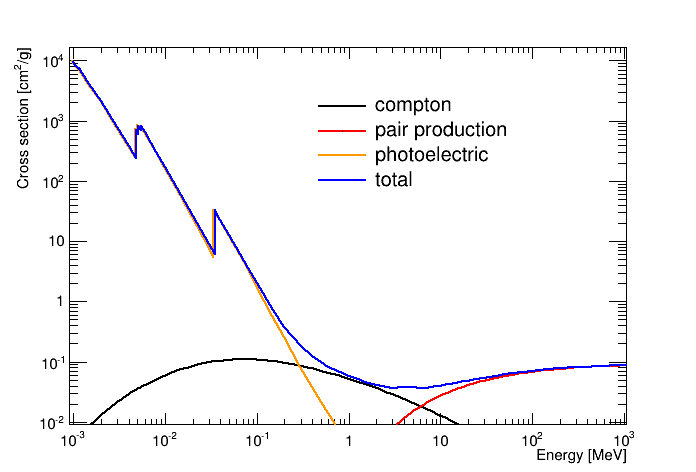
\includegraphics[width=74mm]{Chapter5/figures/xenonGammaXSec.png}
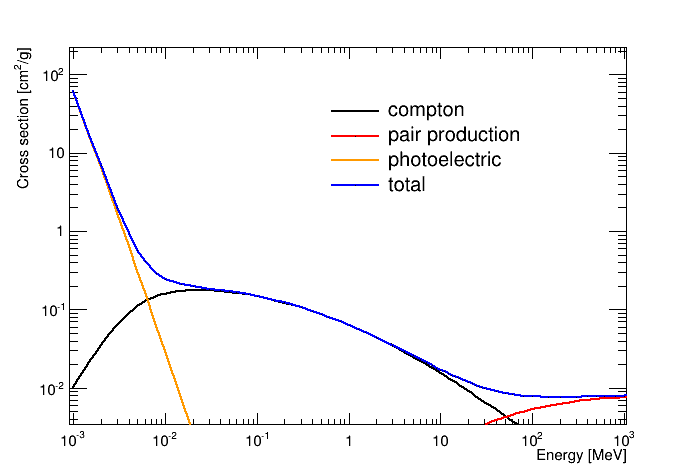
\includegraphics[width=74mm]{Chapter5/figures/heliumGammaXSec.png}
\caption{The cross sections for gamma rays incident on Xe (left) and He (right). Data taken from \cite{nistDatabase}.}
\label{fig:gammaXSecXeHe}
\end{center}
\end{figure}

The critical point of xenon occurs at 289.77 K and 58.41 bar, at this pressure and room temperature (293K) it is in a supercritical phase. Operating a detector in this phase can then be problematic due to strong pressure increases with small temperature increases. Large fluctuations in scintillation light yield also arise due to light propagation in a supercritical fluid. It is therefore favourable to have lower pressures than the neutron detectors to avoid these problems and for the detector to maintain a fairly constant pressure. The isochoric curves for xenon are shown in figure \ref{fig:xenonIsochoric} with the critical point also shown. 

\begin{figure}[htbp]
\begin{center}
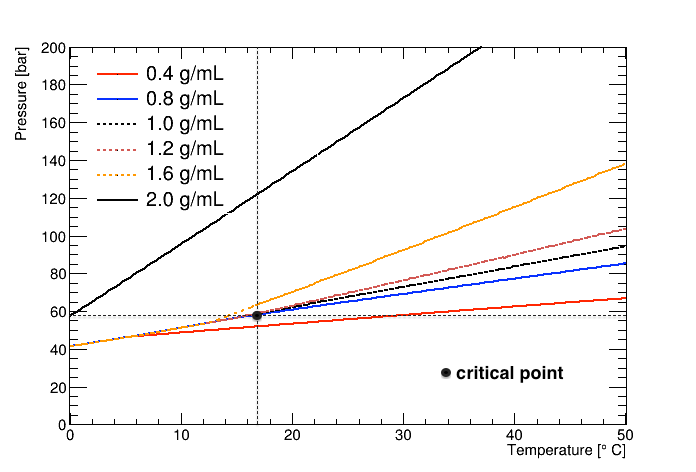
\includegraphics[width=100mm]{Chapter5/figures/xenonIsochoricCurves.png}
\caption{The isochoric curves for xenon at various densities.}
\label{fig:xenonIsochoric}
\end{center}
\end{figure}

The system will need to operate at room temperature, with a total operation range of 0 - 50 $^{\circ}$C, to account for most climates around the world. To avoid the supercritical fluid regime the pressure is set at $\sim$40 bar, corresponding to a density of $\sim$0.3 gcm$^{-3}$ at room temperature. 

The xenon detector has an active volume of $\sim$1570 cm$^{3}$ (10 cm diameter and 20 cm length). Two xenon detectors are proposed for use within the MODES-SNM system.

\subsection{Light Readout}
Hamamatsu R580 PMTs are used for scintillation light readout, with two placed within each detector. An image of the PMTs is shown in figure \ref{fig:ModesPmt}. The spectral response of the R580 PMT lies between 300 to 650 nm, with a peak quantum efficiency of 27\% at 420 nm \cite{hamamatsuPMT}. 

\begin{figure}[htbp]
\begin{center}
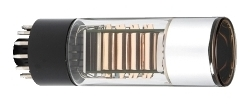
\includegraphics[width=100mm]{Chapter5/figures/hamamatsuPMT.jpg}
\caption{The Hamamatsu R580 Photo Multiplier Tube used in the detectors.}
\label{fig:ModesPmt}
\end{center}
\end{figure}

\subsection{The Electronics System}
The processing of scintillation information, detector monitoring and system power supply is all provided by an electronics system, consisting of five hardware subsystems.

\begin{itemize}
	\item The fully digital Front End electronic system (FE)
	\item The Data Acquisition system (DAQ)
	\item The High Voltage Power Supply system (HV-PS)
	\item The Battery Management System (BMS)
	\item The Information System (IS)
\end{itemize}

\subsubsection{The Front End System}
The FE system acts to digitise the raw scintillation signals from each PMT within the detector assembly. Three 8 channel 14-bit 500 MS/s DT5730 digitisers form the FE system. These units are developed by CAEN specifically for the MODES-SNM project and can be seen in figure \ref{fig:modesDigitisers}. The DT5730 performs analogue to digital conversion with a dead timeless acquisition. After conversion to a digital waveform its internal firmware provides information on timing and pulse charge (energy). Ultimately yielding two charge collection measurements, the short and long components of the digitised waveform, $Q_{short}$ and $Q_{long}$ respectively. These quantities represent the charge collection between the two gates, short (fast component) and long (total), summarised in figure \ref{fig:modesDigitiserGates}. The Pulse Shape Discrimination (PSD) value is then determined from these two parameters, as shown in equation \ref{eq:modesPsdValue}. The PSD value then represents the ratio of the tail to the total integrated spectrum. Due to the different slow component times of neutrons and gammas it is a powerful tool for discrimination between the two particle types. 
%GATE SIZES????

\begin{equation}
	\textnormal{PSD} = (Q_{long} - Q_{short}) / Q_{long} 
	\label{eq:modesPsdValue}
\end{equation}

\begin{figure}[htbp]
\begin{center}
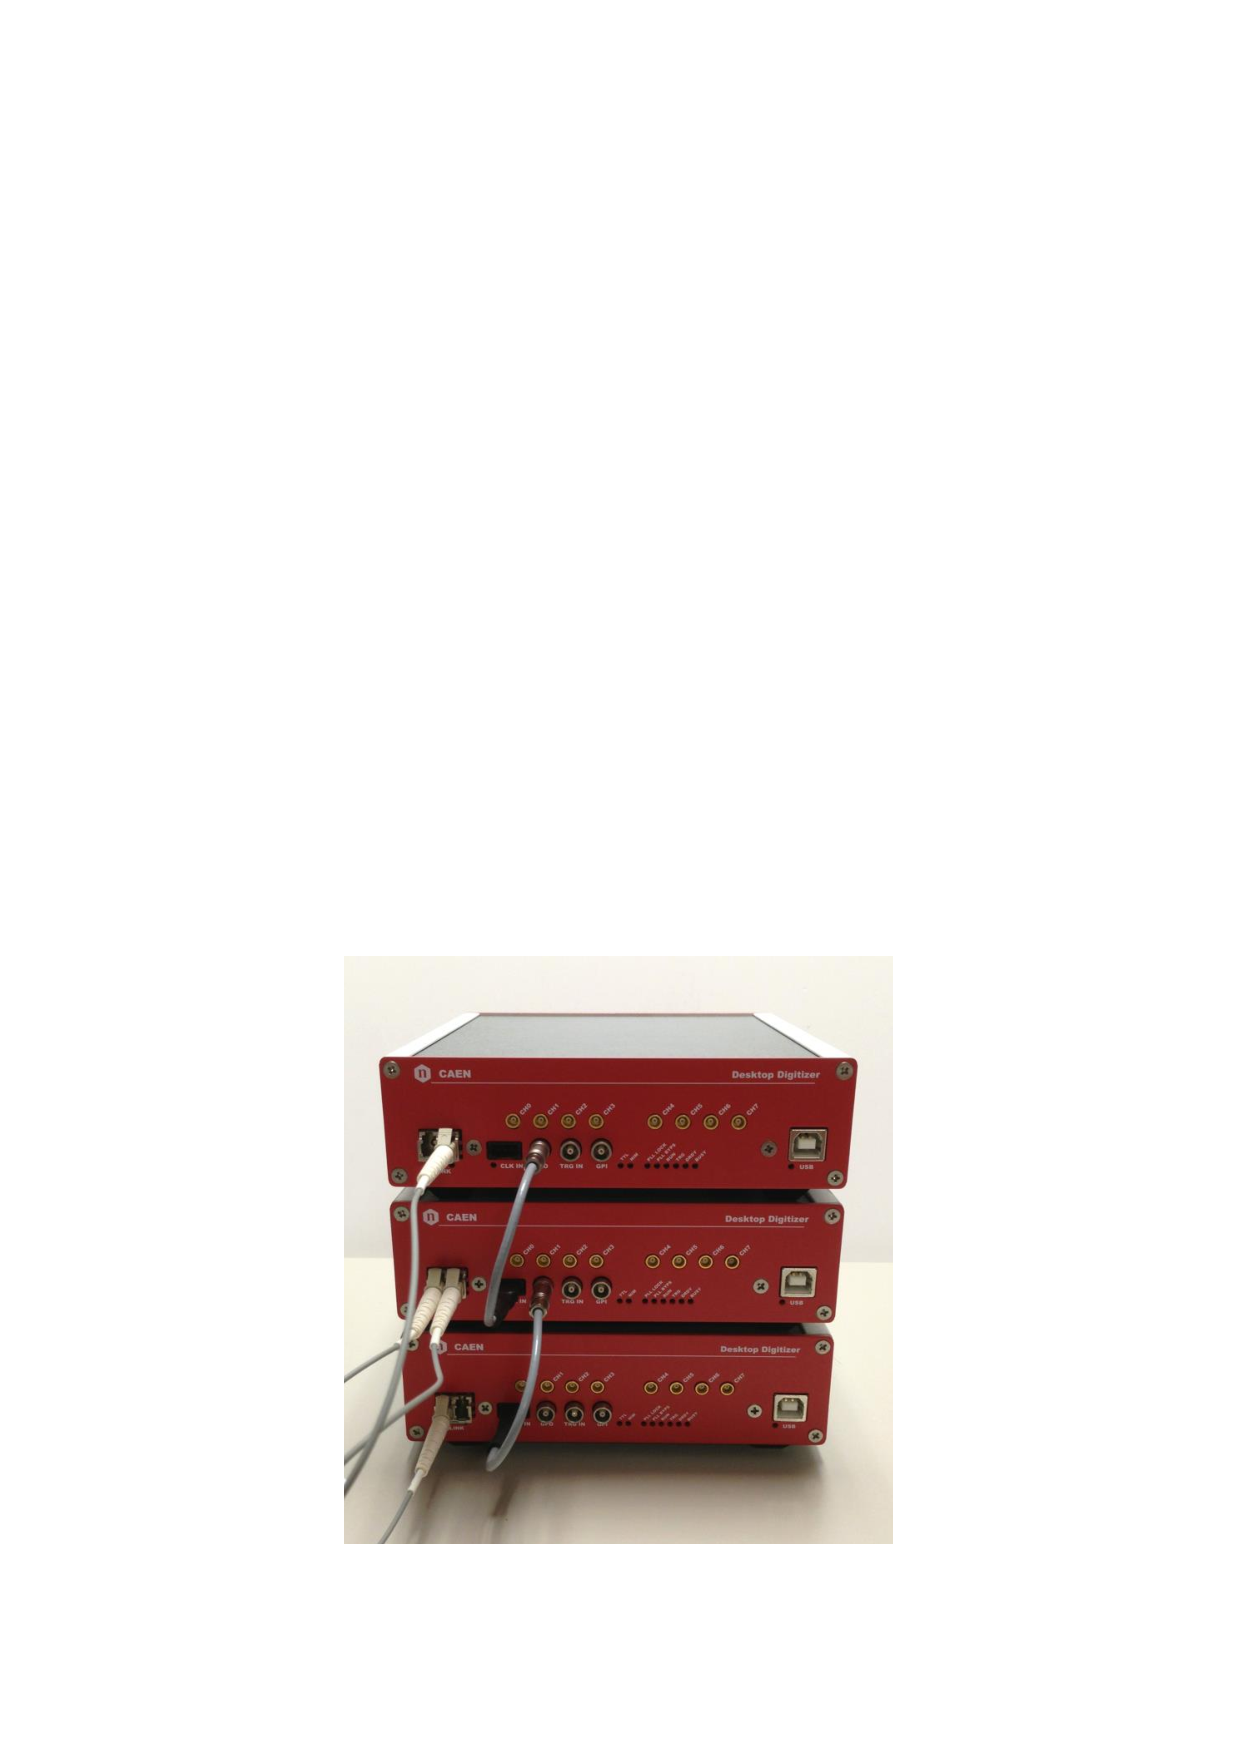
\includegraphics[width=80mm]{Chapter5/figures/digitisers.pdf}
\caption{The three 8 channel 14-bit 500 MS/s DT5730 digitisers that form the FE system. }
\label{fig:modesDigitisers}
\end{center}
\end{figure}

\begin{figure}[htbp]
\begin{center}
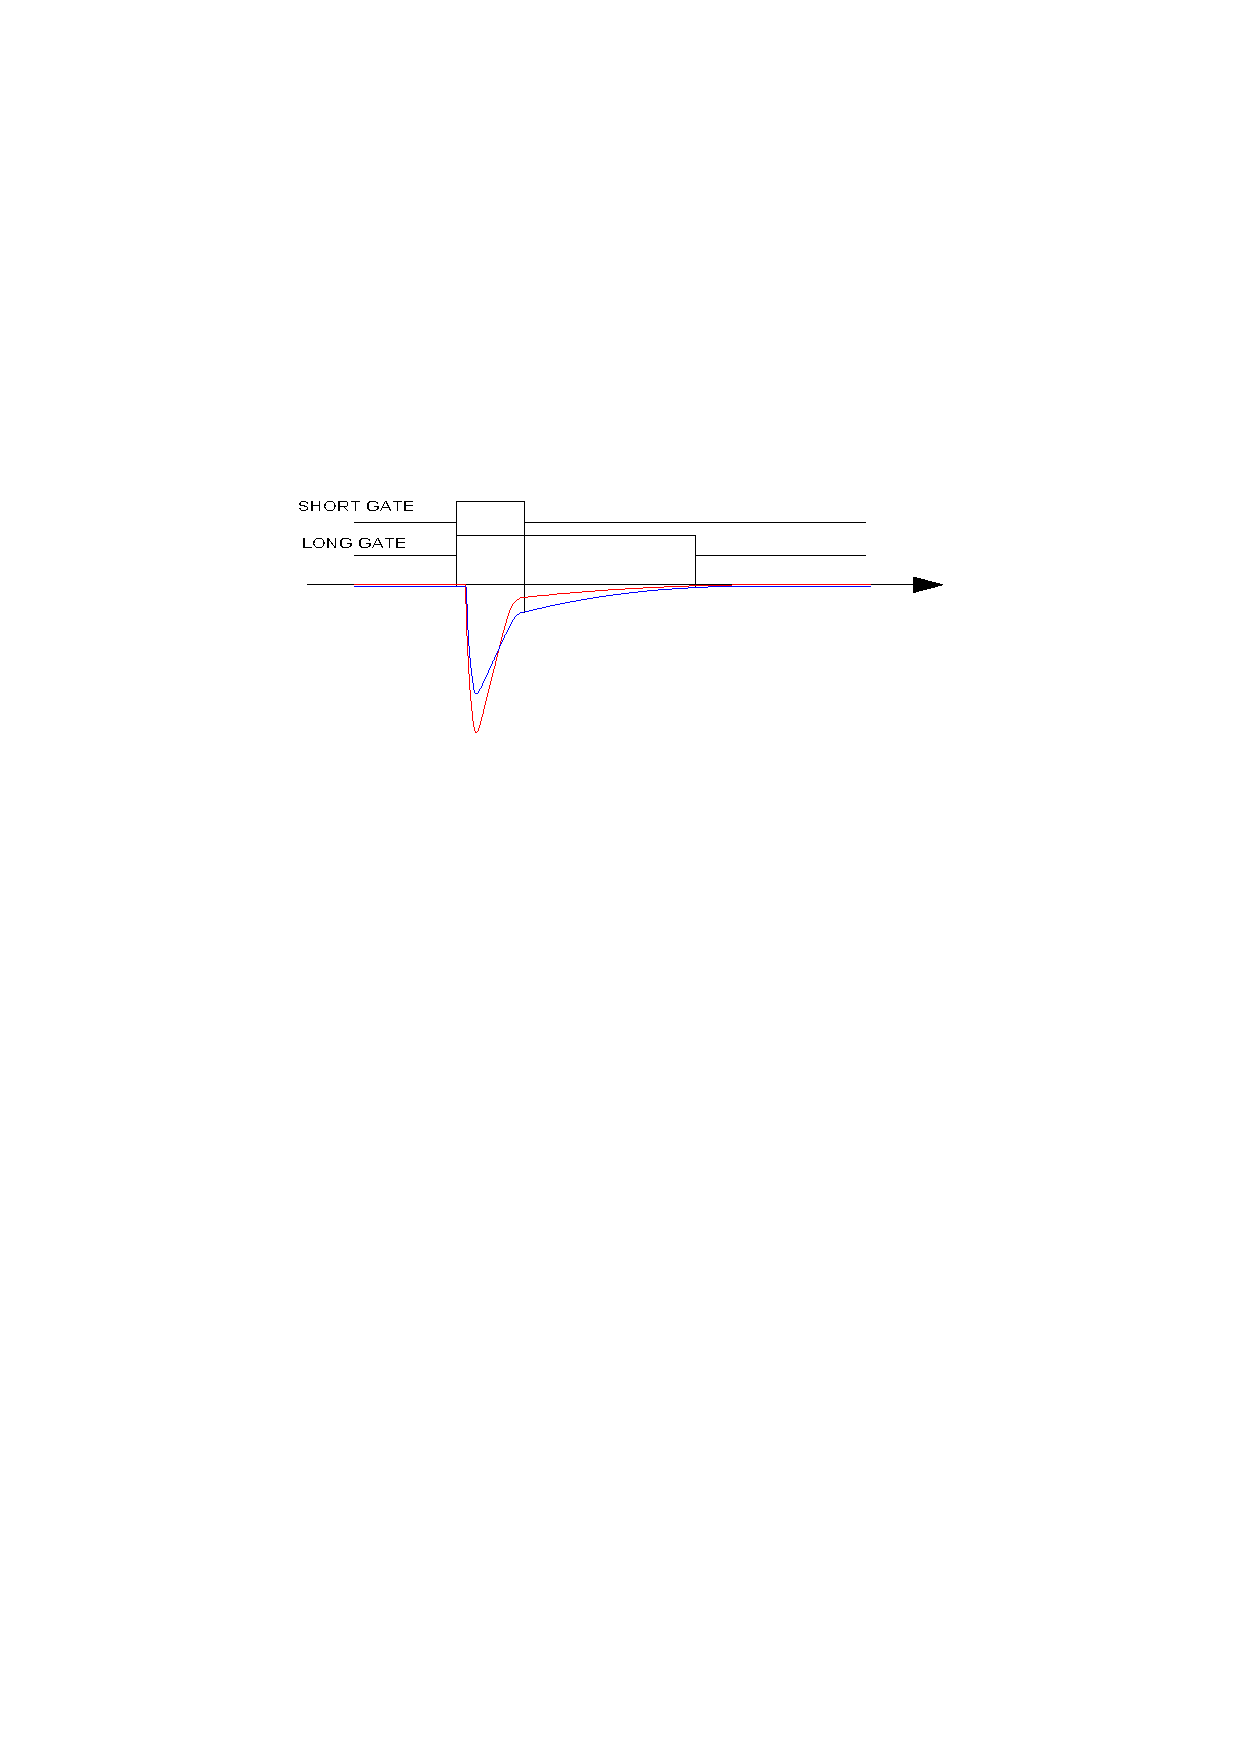
\includegraphics[width=140mm]{Chapter5/figures/digitiserGates.pdf}
\caption{An illustration indicating the two different waveforms with the indications of the short and long gates. Image taken from \cite{modesInternal}}
\label{fig:modesDigitiserGates}
\end{center}
\end{figure}

\subsubsection{The Backend System}
The output from the FE is fed to the DAQ to be processed by the IS. The IS consists of a standard desktop computer (PC) with a Linux based operating system and the bespoke software, designed by University of Padova, already installed. A wireless modem and GPS are connected to the PC in order to communicate with external devices to control the system. The HV-PS is required to provide the necessary high voltages for the PMTs on each detector. The intermediary between the electronics and the battery is the BMS, which monitors and regulates the current and voltage supplied by the battery.

\section{The Software}
The software installed on the IS is designed to process signals from the DAQ, monitor pressures and temperatures of the detectors, while allowing users to manage and control the system. Calibration and data acquisition are also handled by the IS and are integrated into the software. The ROOT package provides the necessary analysis tools required for the system and with the CAEN libraries (used for the FE system) also written in C/C++, a C/C++ framework is a natural choice for the software framework. The software itself is composed of several layers to allow this functionality, this is summarised by figure \ref{fig:modesISSoftware}.

\begin{enumerate}
	\item The control system for data acquisition, the FE system and the HV-PS (FE\&DAQ)
	\item The initialisation and automated calibration process - Setup and Calibration Control System (SU\&CCS)
	\item The decision making algorithms and data analysis (DT)
	\item The graphic user interface - Man Machine Interface (MMI)
\end{enumerate}

\begin{figure}[htbp]
\begin{center}
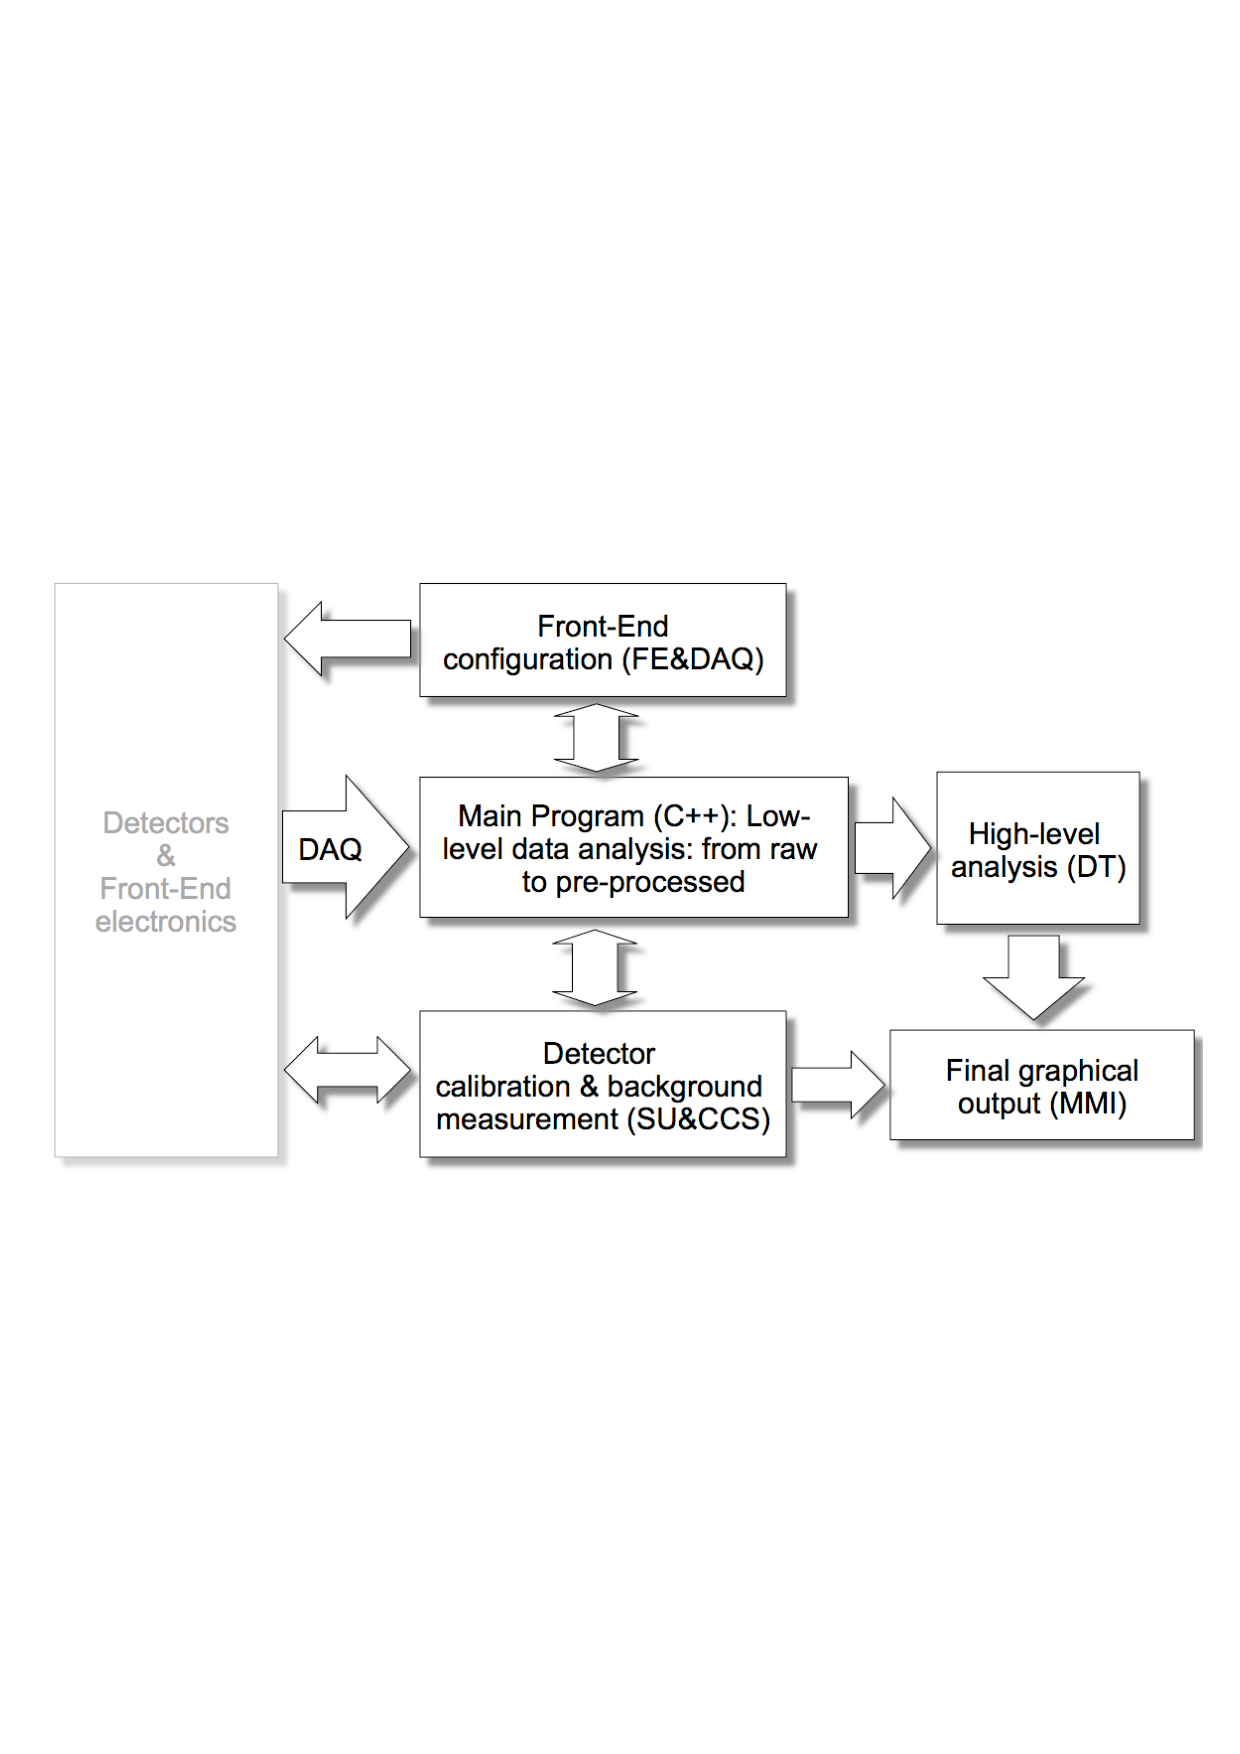
\includegraphics[width=120mm]{Chapter5/figures/IS_softwareStructure.pdf}
\caption{The IS software modular breakdown. Image taken from \cite{modesInternal}}
\label{fig:modesISSoftware}
\end{center}
\end{figure}

\subsection{Uses}
MODES-SNM is not intended to compete with or replace current RPM systems but instead will serve as a selected screening device, to be deployed as a mobile secondary detection unit. This will allow screening on a risk analysis and intelligence basis. However this does not omit it from being deployed as a primary unit and can be used in conjunction with other radioactive detection systems.

The MODES-SNM system will most likely be used at border controls relating to maritime, air, road, rail and postal traffic. These are locations were RPMs are commonly installed. 

It can be easily envisioned that such a system with mobile capabilities would be best deployed for use scanning where threats are occasional and temporary. If deployed with other systems such as X-ray scanners, users would gain additional benefit.

